% \title{Assignment 02 of Automata Theory}

%%%%%%%%%%%%%%%%%%%%%%%%%%%%%%%%%%%%%%%%%
% Short Sectioned Assignment
% LaTeX Template
% Version 1.0 (5/5/12)
%
% This template has been downloaded from:
% http://www.LaTeXTemplates.com
%
% Original author:
% Frits Wenneker (http://www.howtotex.com)
%
% License:
% CC BY-NC-SA 3.0 (http://creativecommons.org/licenses/by-nc-sa/3.0/)
%
%%%%%%%%%%%%%%%%%%%%%%%%%%%%%%%%%%%%%%%%%

% -----------------------------------------------------------------------------
% PACKAGES AND OTHER DOCUMENT CONFIGURATIONS
% -----------------------------------------------------------------------------

\documentclass[paper=a4, fontsize=11pt]{scrartcl} % A4 paper and 11pt font size

\usepackage[T1]{fontenc} % Use 8-bit encoding that has 256 glyphs
\usepackage{fourier} % Use the Adobe Utopia font for the document - comment this line to return to the LaTeX default
\usepackage[english]{babel} % English language/hyphenation
\usepackage{amsmath,amsfonts,amsthm,amssymb} % Math packages
\usepackage{graphicx}

\usepackage{sectsty} % Allows customizing section commands
\allsectionsfont{\centering \normalfont\scshape} % Make all sections centered, the default font and small caps

% --------------------
% Quote Style
% --------------------

\usepackage{tikz}
\usetikzlibrary{backgrounds}
\makeatletter

\tikzset{%
  fancy quotes/.style={
    text width=\fq@width pt,
    align=justify,
    inner sep=.2em,
    anchor=north west,
    minimum width=\textwidth,
  },
  fancy quotes width/.initial={.8\textwidth},
  fancy quotes marks/.style={
    scale=2,
    text=white,
    inner sep=0pt,
  },
  fancy quotes opening/.style={
    fancy quotes marks,
  },
  fancy quotes closing/.style={
    fancy quotes marks,
  },
  fancy quotes background/.style={
    show background rectangle,
    inner frame xsep=0pt,
    background rectangle/.style={
      fill=gray!25,
      rounded corners,
    },
  }
}

\newenvironment{fancyquotes}[1][]{%
  \noindent
  \tikzpicture[fancy quotes background]
  \node[fancy quotes opening,anchor=north west] (fq@ul) at (0,0) {$``$};
  \tikz@scan@one@point\pgfutil@firstofone(fq@ul.east)
  \pgfmathsetmacro{\fq@width}{\textwidth - 2*\pgf@x}
  \node[fancy quotes,#1] (fq@txt) at (fq@ul.north west) \bgroup}
{\egroup;
  \node[overlay,fancy quotes closing,anchor=east] at (fq@txt.south east) {''};
  \endtikzpicture}

\makeatother

% --------------------
% Header and Footer
% --------------------

\usepackage{fancyhdr} % Custom headers and footers
\pagestyle{fancyplain} % Makes all pages in the document conform to the custom headers and footers
\fancyhead[L]{\normalfont \normalsize \textsc{Automata Theory}} % Class
\fancyhead[R]{\normalfont \normalsize \textsc{Wanzhang Sheng}} % Author
\fancyfoot[L]{} % Empty left footer
\fancyfoot[C]{} % Empty center footer
\fancyfoot[R]{\thepage} % Page numbering for right footer
\renewcommand{\headrulewidth}{0pt} % Remove header underlines
\renewcommand{\footrulewidth}{0pt} % Remove footer underlines
\setlength{\headheight}{13.6pt} % Customize the height of the header

\numberwithin{equation}{section} % Number equations within sections (i.e. 1.1, 1.2, 2.1, 2.2 instead of 1, 2, 3, 4)
\numberwithin{figure}{section} % Number figures within sections (i.e. 1.1, 1.2, 2.1, 2.2 instead of 1, 2, 3, 4)
\numberwithin{table}{section} % Number tables within sections (i.e. 1.1, 1.2, 2.1, 2.2 instead of 1, 2, 3, 4)

\setlength\parindent{0pt} % Removes all indentation from paragraphs - comment this line for an assignment with lots of text

% -----------------------------------------------------------------------------
% TITLE SECTION
% -----------------------------------------------------------------------------

\newcommand{\horrule}[1]{\rule{\linewidth}{#1}} % Create horizontal rule command with 1 argument of height

\title{
  \horrule{0.5pt} \\[0.4cm] % Thin top horizontal rule
  \huge Assignment 02 \\ % The assignment title
  \horrule{2pt} \\[1.0cm] % Thick bottom horizontal rule
}

\author{Wanzhang Sheng} % Your name

\date{\normalsize\today} % Today's date or a custom date

\begin{document}

\maketitle % Print the title

% -----------------------------------------------------------------------------
% PROBLEM 1
% -----------------------------------------------------------------------------
\section{}

\begin{fancyquotes}
  For each of the following regular expressions, give a minimum-length string in $(a + b)^*$
  not in the language.
\end{fancyquotes}

\begin{enumerate}
\item (2 points) $b^*(ab)^*a^*$ doesn't match $aab$;
\item (2 points) $(b^*+a^*)(a^*+b^*)(b^*+a^*)$ doesn't match $abab$;
\item (2 points) $a^*(abb^*)b^*$ doesn't match $ba$;
\item (2 points) $b^*(a+ba)^*b^*$ doesn't match $abba$;
\end{enumerate}


% -----------------------------------------------------------------------------
% PROBLEM 2
% -----------------------------------------------------------------------------
\section{}

\begin{fancyquotes}
  Give a regular expression for each of the following languages:
\end{fancyquotes}

\begin{enumerate}
\item (4 points) All strings over $\{a,b\}$ that end in $abb$:
  $$(a+b)^*abb$$
\item (4 points) All strings over $\{a,b\}$ that do not end in $abb$:
  $$(b^*+[a(a+ba+bba)^*bbb]^*)(\epsilon+a+ab)$$ or $$\epsilon + (a+b)^*(a+ab+bbb)$$
\item (4 points) All strings over $\{a,b\}$ that contain the substring $bba$ but not the substring $aa$:
  $$(a+b^*(bb^*a)^*b^*)bbab^*(bb^*a)^*b^*$$
\item (4 points) All strings over $\{0,1\}$ that do not contain the substring $1111$:
  $$0^*(10+110+1110)^*0^*+0^*(1+11+111)$$
\item (4 points) All strings over $\{0,1\}$ that represent binary numbers
$x$, such that $(x \bmod 4) \equiv 1$ (1, 5, 9, 13, etc). Leading zeroes are ok
(so $0000101$ would be in the language, for instance):
  $$(0+1)^*01$$
\end{enumerate}


% -----------------------------------------------------------------------------
% PROBLEM 3
% -----------------------------------------------------------------------------
\section{}

\begin{fancyquotes}
  Give a Deterministic Finite Automaton for each of the following languages:
\end{fancyquotes}

\begin{figure}[hp]
  \centering
  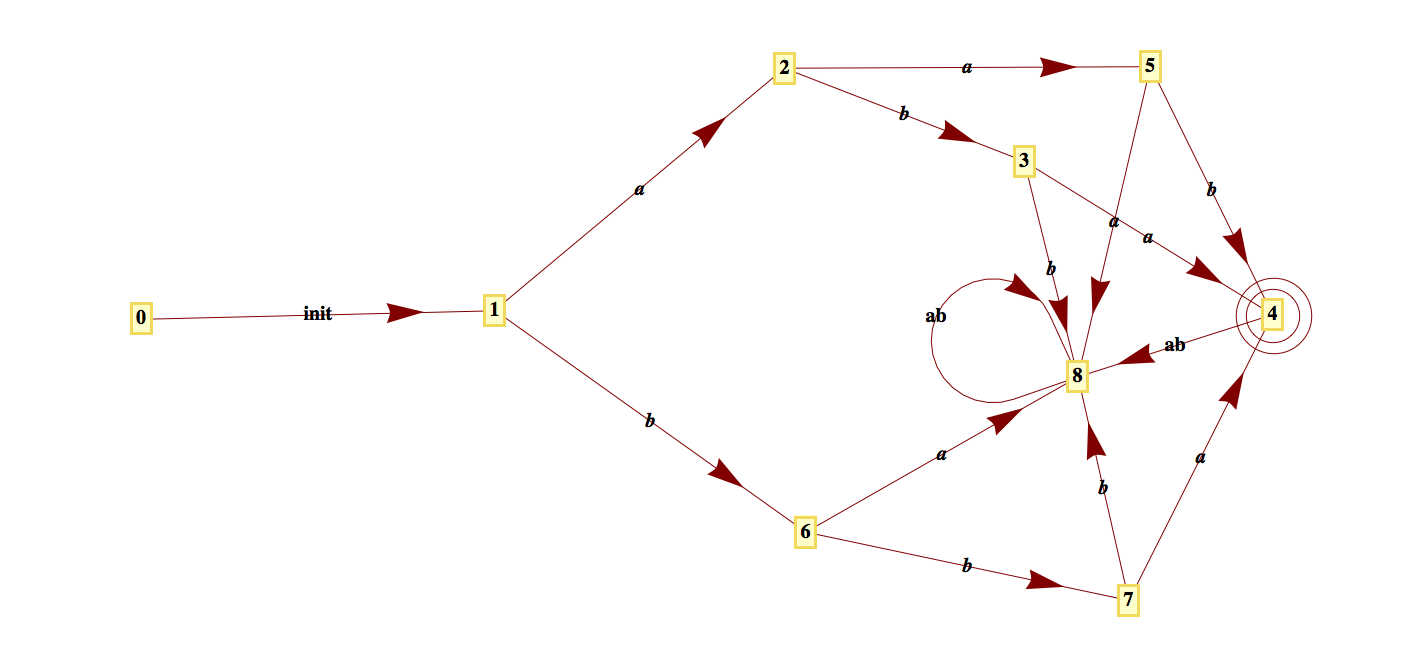
\includegraphics[width=1.0\textwidth]{3-1}
  \caption{The finite language $L=\{aba,bba,aab\}$}
\end{figure}

\begin{figure}[hp]
  \centering
  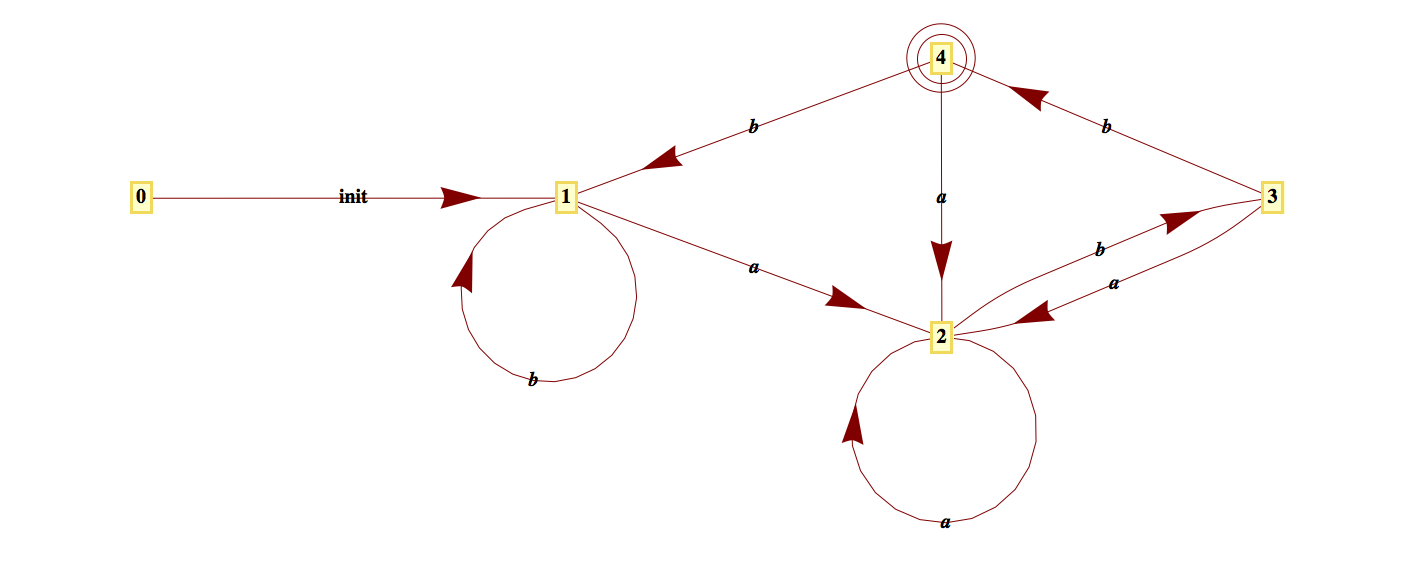
\includegraphics[width=1.0\textwidth]{3-2}
  \caption{All strings over $\{a,b\}$ that end in $abb$}
\end{figure}

\begin{figure}[hp]
  \centering
  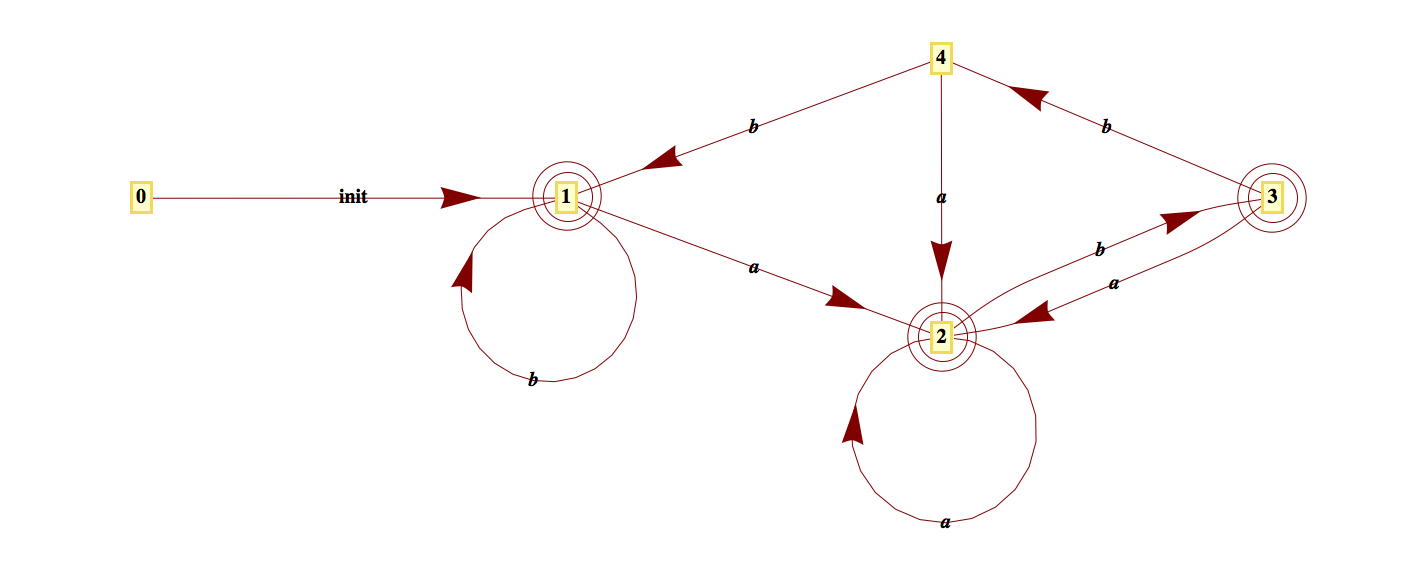
\includegraphics[width=1.0\textwidth]{3-3}
  \caption{All strings over $\{a,b\}$ that do not end in $abb$}
\end{figure}

\begin{figure}[hp]
  \centering
  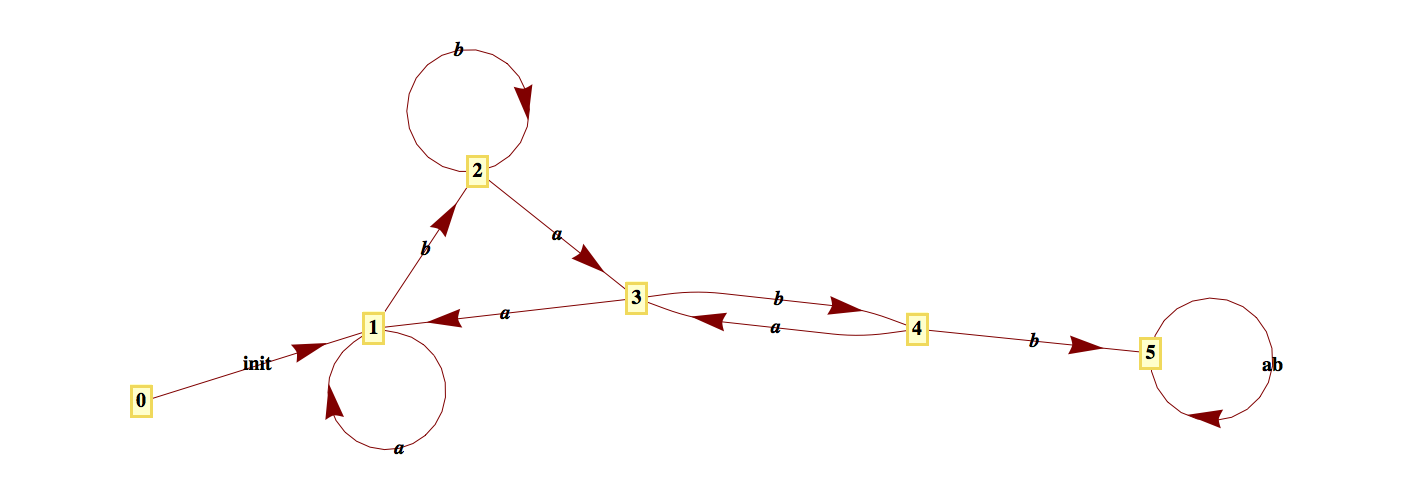
\includegraphics[width=1.0\textwidth]{3-4}
  \caption{All strings over $\{a,b\}$ that contain the substring $babb$}
\end{figure}

\pagebreak

% -----------------------------------------------------------------------------
% PROBLEM 4
% -----------------------------------------------------------------------------
\section{}

\begin{fancyquotes}
  (5 point) Show that every finite language is regular.
\end{fancyquotes}

Considering a finite language $M=(K,\Sigma,\Delta,s,F)$,
which $K={q_1,q_2,q_3,\ldots,q_n}$ and $s=q_1$, $F={q_f,q_{f+1},\ldots,q_n}$.

Define regular languages base on $M$ as: $$R(i,j,k)=\{\omega:
(q_i, \omega) \vdash^*_M (q_j,\epsilon) \between \{q_v: 1\leq v\leq k\} \}$$

For $k=0$, we have:

$$R(i,j,k)=R(i,j,0)=\{\omega: (q_i,\omega) \vdash_M (q_j,\epsilon)\}$$

Base on the result of $k-1$, we can generate the $k$ case as:

$$R(i,j,k)=R(i,j,k-1)\cup R(i,k,k-1)R(k,k,k-1)^*R(k,j,k-1)$$

Therefore $R(i,j,k)$ is regular.

Then we can union the regular languages of all final state:

$$R=\bigcup\{R(1,f,f): f\in F\}$$

So for any finite language, we can find a equivalent regular language:

$$L(M)=L(R)$$

\end{document}
